\section{Date: 2026-07-23}
\noindent \textbf{Series ID: NENUCK9POP} 

\noindent This series is titled Resident Population in Nuckolls County, NE and has a frequency of Annual. The units are Thousands of Persons and the seasonal adjustment is Not Seasonally Adjusted.The observation start date is 1970-01-01 and the observation end date is 2025-01-01.The popularity of this series is 1. \\ 

\noindent \textbf{Series ID: COGANOPIBLEND} 

\noindent This series is titled Medical Services Expenditures by Disease: Other: Congenital Anomalies Price Index, Blended Account Basis and has a frequency of Annual. The units are Index 2017=100 and the seasonal adjustment is Not Seasonally Adjusted.The observation start date is 2000-01-01 and the observation end date is 2021-01-01.The popularity of this series is 1. \\ 

\subsection{Raw Regression}
\noindent Regresses the two series against each other directly. A significant result here can come just as easily from both series sharing a long-run trend as from any real relationship.

\begin{center}
\begin{tabular}{lclc}
\toprule
\textbf{Dep. Variable:}          & value\_fred\_COGANOPIBLEND & \textbf{  R-squared:         } &     0.876   \\
\textbf{Model:}                  &            OLS             & \textbf{  Adj. R-squared:    } &     0.870   \\
\textbf{Method:}                 &       Least Squares        & \textbf{  F-statistic:       } &     141.6   \\
\textbf{Date:}                   &      Thu, 23 Jul 2026      & \textbf{  Prob (F-statistic):} &  1.58e-10   \\
\textbf{Time:}                   &          13:20:04          & \textbf{  Log-Likelihood:    } &   -75.559   \\
\textbf{No. Observations:}       &               22           & \textbf{  AIC:               } &     155.1   \\
\textbf{Df Residuals:}           &               20           & \textbf{  BIC:               } &     157.3   \\
\textbf{Df Model:}               &                1           & \textbf{                     } &             \\
\textbf{Covariance Type:}        &         nonrobust          & \textbf{                     } &             \\
\bottomrule
\end{tabular}
\begin{tabular}{lcccccc}
                                 & \textbf{coef} & \textbf{std err} & \textbf{t} & \textbf{P$> |$t$|$} & \textbf{[0.025} & \textbf{0.975]}  \\
\midrule
\textbf{const}                   &     422.9442  &       28.506     &    14.837  &         0.000        &      363.483    &      482.406     \\
\textbf{value\_fred\_NENUCK9POP} &     -75.7107  &        6.363     &   -11.898  &         0.000        &      -88.985    &      -62.437     \\
\bottomrule
\end{tabular}
\begin{tabular}{lclc}
\textbf{Omnibus:}       &  4.239 & \textbf{  Durbin-Watson:     } &    1.347  \\
\textbf{Prob(Omnibus):} &  0.120 & \textbf{  Jarque-Bera (JB):  } &    2.271  \\
\textbf{Skew:}          &  0.630 & \textbf{  Prob(JB):          } &    0.321  \\
\textbf{Kurtosis:}      &  3.944 & \textbf{  Cond. No.          } &     79.9  \\
\bottomrule
\end{tabular}
%\caption{OLS Regression Results}
\end{center}

Notes: \newline
 [1] Standard Errors assume that the covariance matrix of the errors is correctly specified.

\begin{figure}
\centering
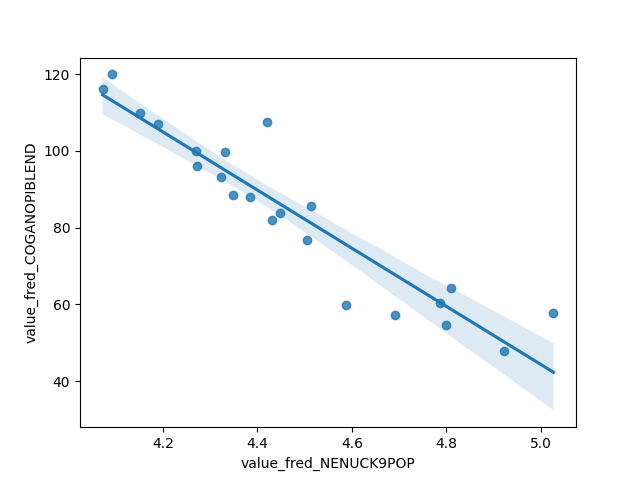
\includegraphics[scale = 0.9]{plots/plot_2026-07-23.png}
\caption{Raw Regression Plot for 2026-07-23}
\end{figure}
\newpage
\subsection{Detrended Regression}
\noindent Regresses the residuals of each series after removing its own linear time trend, so a shared trend can no longer drive the result on its own. A relationship that stays significant here is better evidence of a genuine link between the two series.

\begin{center}
\begin{tabular}{lclc}
\toprule
\textbf{Dep. Variable:}                     & value\_fred\_COGANOPIBLEND\_detrended & \textbf{  R-squared:         } &     0.358   \\
\textbf{Model:}                             &                  OLS                  & \textbf{  Adj. R-squared:    } &     0.326   \\
\textbf{Method:}                            &             Least Squares             & \textbf{  F-statistic:       } &     11.17   \\
\textbf{Date:}                              &            Thu, 23 Jul 2026           & \textbf{  Prob (F-statistic):} &  0.00324    \\
\textbf{Time:}                              &                13:20:05               & \textbf{  Log-Likelihood:    } &   -75.552   \\
\textbf{No. Observations:}                  &                     22                & \textbf{  AIC:               } &     155.1   \\
\textbf{Df Residuals:}                      &                     20                & \textbf{  BIC:               } &     157.3   \\
\textbf{Df Model:}                          &                      1                & \textbf{                     } &             \\
\textbf{Covariance Type:}                   &               nonrobust               & \textbf{                     } &             \\
\bottomrule
\end{tabular}
\begin{tabular}{lcccccc}
                                            & \textbf{coef} & \textbf{std err} & \textbf{t} & \textbf{P$> |$t$|$} & \textbf{[0.025} & \textbf{0.975]}  \\
\midrule
\textbf{const}                              &    6.695e-12  &        1.678     &  3.99e-12  &         1.000        &       -3.499    &        3.499     \\
\textbf{value\_fred\_NENUCK9POP\_detrended} &     -78.2472  &       23.407     &    -3.343  &         0.003        &     -127.074    &      -29.421     \\
\bottomrule
\end{tabular}
\begin{tabular}{lclc}
\textbf{Omnibus:}       &  3.865 & \textbf{  Durbin-Watson:     } &    1.355  \\
\textbf{Prob(Omnibus):} &  0.145 & \textbf{  Jarque-Bera (JB):  } &    1.985  \\
\textbf{Skew:}          &  0.584 & \textbf{  Prob(JB):          } &    0.371  \\
\textbf{Kurtosis:}      &  3.896 & \textbf{  Cond. No.          } &     14.0  \\
\bottomrule
\end{tabular}
%\caption{OLS Regression Results}
\end{center}

Notes: \newline
 [1] Standard Errors assume that the covariance matrix of the errors is correctly specified.

\begin{figure}
\centering
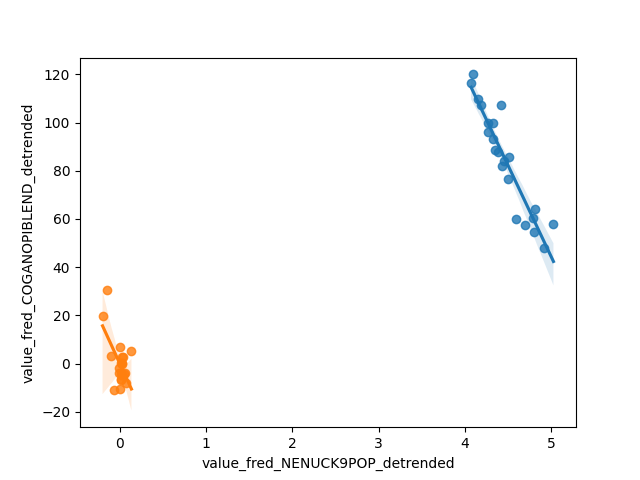
\includegraphics[scale = 0.9]{plots/plot_2026-07-23_detrended.png}
\caption{Detrended Regression Plot for 2026-07-23}
\end{figure}
\newpage
